\chapter{Introduction}
\section{Overview}
%https://nsdsguidelines.paris21.org/node/291
%https://papers.ssrn.com/sol3/papers.cfm?abstract_id=2622220


%markets:
%https://link.springer.com/article/10.1007/s10551-010-0402-8
%https://www.oecd-ilibrary.org/content/paper/5k49dfg9fb6d-en

Almost two billion people live in states characterized as fragile. These fragile states are characterized by weak state capacity, leaving its citizens vulnerable to various shocks, and unable to the benefit from the growing world wide prosperity. %expand




\section{Conceptual Framework}


The chapters of this thesis are intended as separate contributions about the impacts of these characteristics on development. The focus lies on the impact on institutions and social capital; behaviour; productivity; and human rights. 

%list of what the thesis does.



%Social Capital and Instutions
%Rodrik2004
\subsection{Social Capital, Institutions and Development}
The key factor that sets apart Fragile States from their more stable counterparts, is the institutional environment \cite{Rodrik2004,Acemoglu2000}. This term is used to describe the way in which (economic) life is organized. It covers crucial things such as protection of property rights and equal treatment by the law \citep{Acemoglu2005}. Such good institutions incentivize innovation The relationship between institutions and growth does not run in one direction: economic growth allows for better institutions and vice versa. But is clear that improved institutions cause additional growth \cite{Acemoglu2000}.

A second important factor to economic growth is cooperative behaviour. Especially in poorer countries, trust plays an important role in facilitating economic activity \citep{Knack1997}. In such countries, trust and social capital may be a substitute for formal institutions to incentivize innovation by providing insurance and securing property rights. However, institutions can also increase cooperative behaviour \cite{Bo2008,Henrich2010}. This implies that countries with either cooperative behaviour or good institutions can enter a virtuous cycle of institutions producing growth and cooperative behaviour; and cooperative behaviour and growth producing quality institutions.

The question on how to enable such a virtuous cycles for fragile states is too large for any one thesis. This thesis provides empirical, micro-level level evidence on how social capital and behaviour mediate development in fragile states. Figure \ref{fig:intro_framework} outlines these concepts. 

figures
\begin{figure}[htb]
  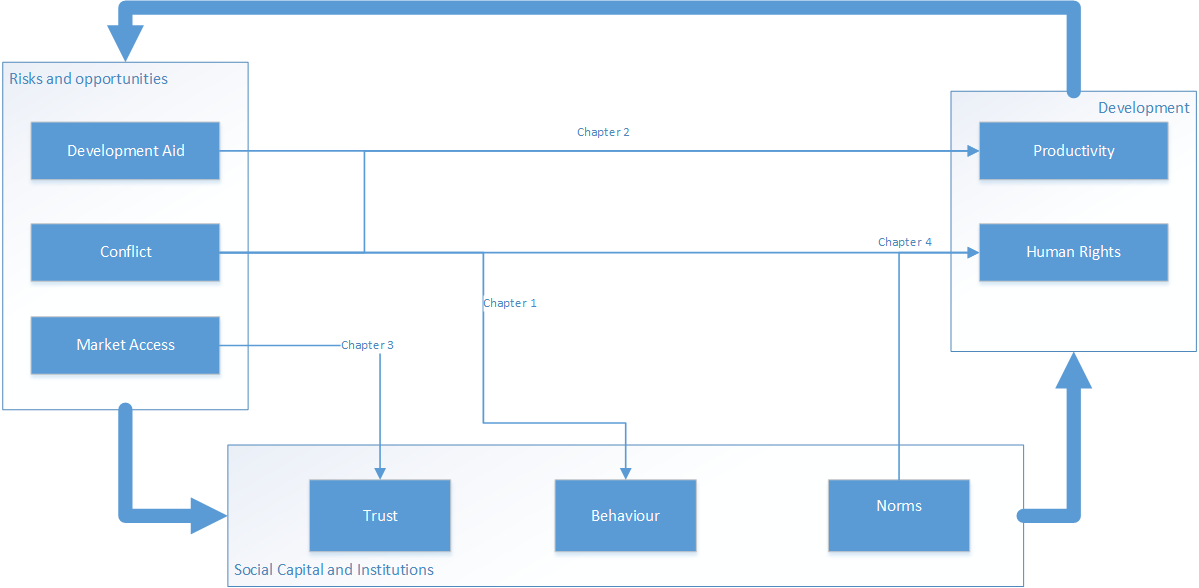
\includegraphics[width=0.8\linewidth]{"C:/Users/Koen/Documents/GitHub/thesis/figures/introduction/conceptual_framework.png"}
  \caption{Conceptual Framework}
  \label{fig:intro_framework}
\end{figure}


I focus on three separate characteristics of Fragile States, that either present risks or oppurtunities for their development. Firstly, they are frequently settings for violent conflict. SOME STATISTICS MAYBE? Secondly, they are poorly connected to world markets. This leads to a lack of opportunities for exchange and specialization, and underwhelming economic development. Thirdly, Fragile States are large recipients of development aid. The lack of state capacity makes it hard to fulfil citizen's needs for healthcare, education, and services, leading to international donors to attempt and alleviate the resulting humanitarian crises. 

As for development, I focus on human rights, and agricultural productivity. MOTIVATE.

The questions this thesis aims to answer are:
\begin{enumerate}
	\item What is the relationship between conflict and competitive behaviour? (Chapter 1);
	\item What is the effect of input subsidies on novel technology adoption? (Chapter 2);
	\item What is the effect of market access on trusting behaviour; and,
	\item What are the drivers of sexual and gender-based violence in Eastern Congo (Chapter 3).
\end{enumerate}



%Trust and civic norms are stronger in nations with higher and more equal incomes, 


%Productivity


%Human Rights


%Agricultural Productivity

%football paper.
The first chapter explores the relationship between conflict and behaviour. %SOME KEY SENTENCES HERE. 

The second paper focuses more on the international community's 
%


Here I focus on three important characteristics of Fragile States: Fragile States are poorly connected to markets; ; and they are among the world's largest recipients of development aid. This thesis focuses on the effects that these three characteristics have on the daily lives of the citizens of Fragile States. The aspects of daily life I focus on are: Social Capital and Institutions; Productivity; Behaviour; and Human Rights.

The first chapter explores the impacts of conflict on behaviour. 



\section{Contribution}


\section{Outline}


%bibliography, this is needed for bibtex
\clearpage 
\bibliographystyle{chicago}
%path to .bib file (e.g. automatically exported by mendeley) DO NOT include the file extension!
\bibliography{C:/Users/Koen/Dropbox/Literatuur/Mendeley/Bibtex/Thesis-Introduction}